\chapter{绪\hspace{1em}论}
\label{ch1:intro}

\section{引言}
LUT \LaTeX~Template: LuThesis v1.1。

该模板为兰州理工大学硕士学位论文模板,基于 ThuThesis LATEX Template 修改,Author: Yang Guoqiang,Email: estivalinp@163.com。该模板提供基本的文档元素例子,更复杂的例子请参考硕士论文:《杨国强\_车间调度问题的适应度地形及智能优化算法研究》。

注意:使用该模板时,段落之间请空一行。脚注示例\footnote{这是一个脚注。This is a footnote.}。

\section{使用展示}

\subsection{插入一幅图}

例如,图 \ref{fig:ch1:flowchat} 为制造系统中的信息流图。
\begin{figure}%[H] % use float package if you want it here
	\centering
	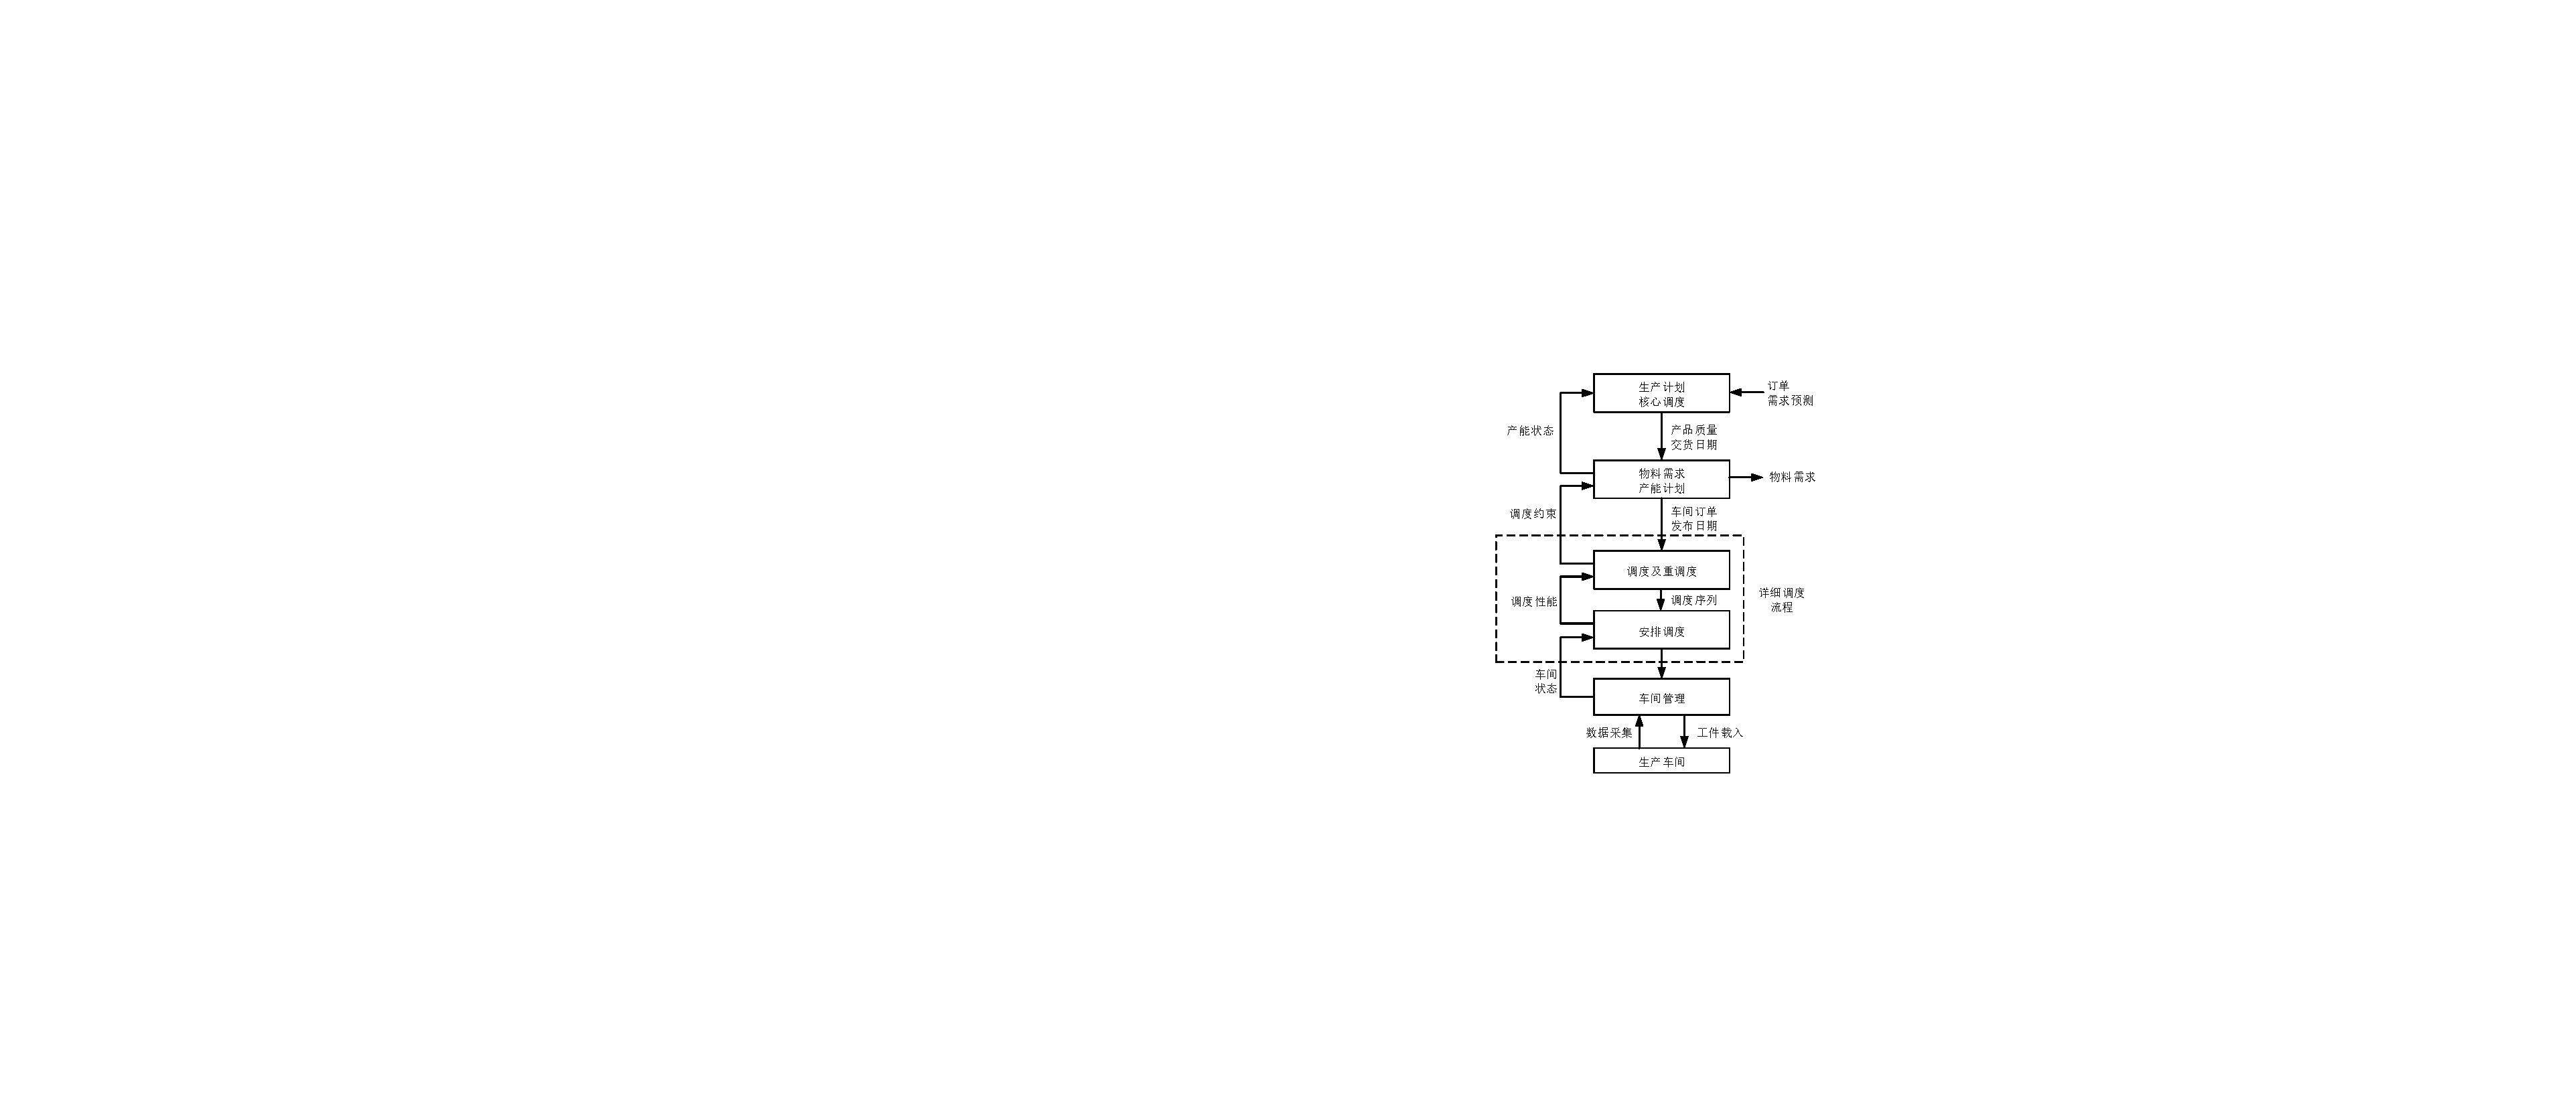
\includegraphics{fig_ch1_flowchat}
	\caption{制造系统中的信息流图}
	\label{fig:ch1:flowchat}
\end{figure}

\subsection{插入一张表}

例如,对应的映射关系如表~\ref{tab:ch2:mapping} 所示。
\begin{table}[htbp]
	\wuhao\centering
		\caption{工件序列、阶乘因子串及阶乘数之间的映射关系$(n=3)$}
		\label{tab:ch2:mapping}
		\begin{tabular}{m{4cm}<{\centering}m{4cm}<{\centering}m{4cm}<{\centering}}
			\toprule[1.5pt]
			工件序列 & 阶乘因子串 & 阶乘数(十进制形式)\\%\tabincell{c}{阶乘数\\(十进制形式)} \\
			\midrule[0.5pt]
			\{1, 2, 3\} & \{0, 0, 0\} & 0\\
			\{1, 3, 2\} & \{0, 1, 0\} & 1\\
			\{2, 1, 3\} & \{1, 0, 0\} & 2\\
			\{2, 3, 1\} & \{1, 1, 0\} & 3\\
			\{3, 1, 2\} & \{2, 0, 0\} & 4\\
			\{3, 2, 1\} & \{2, 1, 0\} & 5\\
			\bottomrule[1.5pt]
		\end{tabular}
\end{table}

\subsection{插入一个行间公式}

例如,最后一台机器上的两个相邻工件完成时间之差 $d_{j-1,j}$ 可由公式(\ref{equ:chap1:distence})算得。

注意,模板中正文与begin{equation}之间不能存在空行,{\heiti 这是正文中的黑体}。
\begin{equation}
	\label{equ:chap1:distence}
	\begin{aligned}
	d_{j-i,j}=C_{i,m}-C_{j-i,m}&=\sum_{k=1}^{i}{p_{j,k}}-\min\limits_{1 \leq i \leq m}\big(\sum_{k=1}^{i-1}{p_{j,k}}+\sum_{k=i+1}^{m}{p_{j-1,k}}\big)\\
	&=\max\limits_{1 \leq i \leq m}\big(\sum_{k=1}^{m}{p_{j,k}}+\sum_{k=1}^{i-1}{p_{j,k}}-\sum_{k=i+1}^{m}{p_{j-1,k}}\big)\\
	&=\max\limits_{1 \leq i \leq m}\big(\sum_{k=1}^{m}{p_{j,k}}-\sum_{k=i+1}^{m}{p_{j-1,k}}\big)
	\end{aligned}
\end{equation}

\subsection{插入一个算法}

例如,算法 \ref{alg:ch2:encoding} 给出了阶乘数的详细编码过程。

\begin{myAlgorithm}
	\setstretch{1}
    \caption{阶乘数编码算法} %\strut
    \label{alg:ch2:encoding}
    \KwIn{Job permutation $\pi=\{J_1,J_2,\cdots,J_{j-1},J_j,\cdots,J_n\} $\;}
    \KwOut{Natural number $ N_F $\;}
    \textbf{Initialize: }$ D_F=\{0,1,\cdots,n-1\} $, $ P=\{1,2,\cdots,n\} $, $ F=\varnothing $, $  N_F=0 $\;
    \For {$j \gets 1;j \leqslant n;j \ne i$}
    {
		 \algolines{$ index \gets Find(P[index]==J_i) $}{Find the first position index from left to right in $ P $ which makes $ P[index] $ equal to $ J_i $.}
		 $F[i] \gets D_F [index]$\;
		 remove $ P[index] $ from $ P $\;
		 $ N_F \gets N_F+F[i] \times D_F [n-i+1]! $\;
    }
    \Return{$ N_F $}
\end{myAlgorithm}

\subsection{定理及证明}

本文使用Markov模型对HILS的收敛性进行分析。本文使用的依概率收敛定义如下:

\begin{definition}
	(依概率收敛\textsuperscript{[160]})设 $ \{x(t),t=0,1,2 \cdots \} $ 为基于种群的随机算法产生的种群随机序列。称随机序列 $ \{x(t)\} $ 依概率弱收敛于全局最优,当且仅当:	
	\begin{equation}
		\label{equ:chap5:equation1}
		\lim_{t \to +\infty}P\{x(t) \cap B^* \neq \varnothing\}=1
	\end{equation}
	
	\noindent 其中 $ B^* $ 为优化问题的全局最优解。
\end{definition}
	
\begin{nature}
	对于不包含SHADE中选择算子的HILS,其种群空间 $ \varPhi^m $ 的所有状态(种群)都是连通的。对于所有状态 $ X,Y \in \varPhi^m $,从 $ X $ 到 $ Y $ 的一步转移概率大于0。即:
	\begin{equation}
		\label{equ:chap5:nature1}
		P\{A^0 \cdot L^0 \cdot P^0 (X)=Y\}>0. 
	\end{equation}
\end{nature}

\begin{theorem}
	\label{sec:theorem}
	假设 $ \{x(t),t=0,1,2 \cdots\} $ 为HILS迭代过程中的种群序列,则 $ \{x(t),t=0,1,2 \cdots\} $ 能依概率收敛到全局最优。
\end{theorem}

\begin{proof}
	对于不包含SHADE中选择算子的HILS,仅存在三个算子:扰动算子 $ P^0 $,局部搜索算子$  L^0 $ 和接受准则算子 $ A^0 $。又因为 $ e^{- \Delta f / T_G}>0 $,所以:
	\begin{equation}
		\label{equ:chap5:proof1_3}
		e^{- \Delta f/T_G}  \cdot \sum_{Z \in \varPhi^m}P\{L^0 \cdot P^0 (X)=Z\} \cdot P\{A^0 (X,Z)=Y\}>0.
	\end{equation}
	
	\noindent (这是不缩进的一段)即,对于不包含SHADE中选择算子的HILS而言,从任意状态 $ X $ 到任意状态 $ Y $ 的一步转换概率大于0。因此,对于没有选择算子的HILS,所有种群状态都是连续的。\hfill $ \square $
\end{proof}

\subsection{条、款的使用}

\begin{enumerate}
	\item 第一条第一条第一条第一条第一条第一条第一条第一条第一条第一条第一条第一条第一条第一条第一条第一条第一条第一条第一条第一条第一条第一条第一条第一条第一条第一条第一条第一条第一条第一条第一条第一条第一条第一条第一条第一条第一条第一条第一条。
	\begin{itemize}[itemsep=0ex,partopsep=0pt,parsep=0ex,topsep=6bp,labelsep=10pt]
		\item 第一款第一款第一款第一款第一款第一款第一款第一款第一款第一款第一款第一款第一款第一款第一款第一款第一款;
		\item 第二款第二款第二款第二款第二款第二款第二款第二款第二款第二款第二款第二款第二款第二款第二款第二款第二款;
		\item 第三款第三款第三款第三款第三款第三款第三款第三款第三款第三款第三款第三款第三款第三款第三款第三款第三款。
	\end{itemize}
	\item 第二条第二条第二条第二条第二条第二条第二条第二条第二条第二条第二条第二条第二条第二条第二条第二条第二条第二条第二条第二条第二条第二条第二条第二条第二条第二条第二条第二条第二条第二条第二条第二条第二条第二条第二条第二条第二条第二条第二条。
	\item 第三条第三条第三条第三条第三条第三条第三条第三条第三条第三条第三条第三条第三条第三条第三条第三条第三条第三条第三条第三条第三条第三条第三条第三条第三条第三条第三条第三条第三条第三条第三条第三条第三条第三条第三条第三条第三条第三条第三条。
\end{enumerate}

\section{本论文的主要研究内容及创新之处}
***

\section{本论文的组织安排}
***
